\documentclass[10pt,a4paper]{article}
\usepackage[utf8]{inputenc}
\usepackage[french]{babel}
\usepackage[T1]{fontenc}
\usepackage{lmodern}
\usepackage{amsmath}
\usepackage{amsfonts}
\usepackage{amssymb}
\usepackage{graphicx}
\usepackage{subfigure}
\usepackage{subfig}
\usepackage{natbib}
\usepackage{layout}
\usepackage{wrapfig}
\usepackage{minitoc}
\usepackage{url}
%\usepackage{caption}
%\usepackage{subcaption}

\usepackage[top=1.5cm,bottom=1.5cm,left=1.5cm,right=1.5cm]{geometry}
\usepackage{listings}

\author{Philippe Verbist - Antoine Paris \\ \ \ \ 3521-13-00\ \ \ \ \ \ 3158-13-00}
\title{\textbf{Rapport du projet DJ'Oz}}
\date{Le 4 décembre 2014}
\begin{document}
\sloppy
\maketitle

\paragraph{Remarque importante}
Si la compilation prend trop de temps (environ 4 minutes), il existe une version
\textit{sobre} de nos musiques (sans les instruments, ce qui diminue le temps
de compilation à seulement 14 secondes). Pour charger cette version
sobre, il suffit de remplacer la dernière ligne du fichier exemple.dj.oz
par la ligne juste au dessus (qui normalement est en commentaire).
Enfin, le fichier out.wav correspondant à la version original
est inclus dans notre soumission.

\section{Structure du programme}
Comme il nous l'a été demandé, nous avons divisé notre programme en trois parties:
\begin{itemize}
	\item une fonction Interprete, qui prend une partition en paramètre et renvoie une liste d'échantillons;
	\item une fonction Mix, qui 1) prend en paramètre une fonction qui permet d'interpréter une partition 
	et une musique et qui  2) renvoie un vecteur audio, sous la forme d'une liste de flottants compris dans l'intervalle [-1.0;1.0];
	\item un fichier example.dj.oz, qui contient une musique.
\end{itemize}
\vspace{0.5 cm}

Le tableau suivant reprend de manière synthétique la structure de nos deux fonctions.

\begin{center}
		\begin{tabular}{|p{0.10\textwidth}|p{0.22\textwidth}|p{0.25\textwidth}|p{0.25\textwidth}|}
		\hline
		\textbf{Fonction}		& \textbf{Sous-fonction maîtresse} 	& \textbf{Sous-fonctions principales} 										& \textbf{Autres sous-fonctions}	\\
		\hline
		Interprete					& InterpreteFlattened								& DureeTrans, Etirer, Bourdon, Transpose, Instrument, ... & ToNote, NumberOfSemiTones, ...	\\
		\hline
		Mix 								& MixMusic 													& MixVoice, Merge, RepetitionNB, Echo, ... 								&  Fill, Combine, ...							\\
		\hline 
		\end{tabular}
\end{center}
	
\section{Décisions de conception et astuces de programmation}
\paragraph{Programmation déclarative} 
Aucune structure non-déclarative ne s'est avérée nécessaire
pour écrire notre programme ; nous n'en avons donc pas utilisé.

\paragraph{Récursion terminale} 
Afin de rendre notre code plus rapide, nous avons fait en 
sorte que toutes nos sous-fonctions soient récursives terminales. 
Pour ce faire, nous avons, notamment, utilisé des accumulateurs.
 
\paragraph{Privilégier autant que possible l'appel de fonctions déjà créées} 
Une des grandes difficultés du projet a été l'\textit{imbrication} de données dans d'autres données. 
Par exemple, une musique peut contenir un filtre, qui contient un filtre,
qui contient un merge, qui contient une musique, qui contient une partition, qui contient une transformation, ... 
Pour pouvoir faire sortir progressivement tout ces différents niveaux de données, nous avons systématiquement ré-appelé
la fonction maîtresse dans chaque sous-fonction secondaire.

\paragraph{Astuce lors des récursions}
A de nombreux endroits du code, nous avons dû construire progressivement une liste. 
Lorsque l'on utilise un accumulateur, une technique  consiste à utiliser la fonction 
\{Append Accumulateur NouvelElement\}. La difficulté est que Append  parcourt tout 
l'accumulateur avant "d'ajouter" le nouvel élément. Or, très souvent, l'accumulateur 
est très grand - en particulier si la musique à mixer est grande - et le nouvel élément,
très petit (il s'agit, très souvent, d'un seul élément). Pour accélérer notre code, 
nous inversons donc les arguments: \{Append NouvelElement Accumulateur\}, et à la fin 
de la fonction, nous renvoyons \{Reverse Accumulateur\}. Ceci permet de ne parcourir 
qu'une seule fois l'accumulateur en entier, et donc de réduire la complexité temporelle
de la fonction de $\mathcal{O}(n!)$ à $\mathcal{O}(n)$. Cette technique s'est avérée particulièrement efficace
lorsque nous devions construire un vecteur audio d'une certaine fréquence (fonction Fill),
dont la longueur moyenne est de 44 100 éléments (ce qui correspond à 1 seconde).

\paragraph{Astuce lors de Reverse :} 
l'astuce précédente, bien qu'elle permet d'accélérer grandement nos fonctions, a amené un problème :
si NouvelElement est une liste, alors non seulement les éléments ne seront plus dans l'ordre,
mais en plus il sera impossible de les reclasser dans le bon ordre en appelant \{Reverse Acc\}. 
Pour corriger ce problème, nous avons  créé une liste de listes (voir Figure \ref{fig:astuceReverse}), 
et, ensuite, renvoyé la liste \{Flatten \{Reverse Acc\}\}.

\begin{figure}[h!]
	\centering
	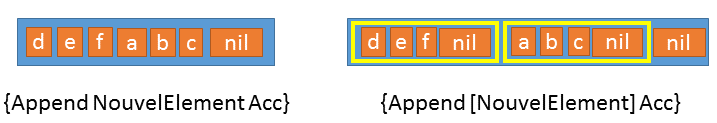
\includegraphics[width=10cm]{images/AstuceAppend.png}
	\caption{A gauche : une liste qu'il est impossible de reclasser dans le bon ordre. 
	A droite : une liste de listes qu'il est possible de reclasser dans le bon ordre en appelant Reverse.}
	\label{fig:astuceReverse}
\end{figure}

\section{Complexité calculatoire}
Dans cette section, nous donnons les complexité calculatoire
propre de chaque fonction, c'est à dire sans tenir des sous-fonctions
utilisées.

\begin{center}
		\begin{tabular}{|l|l|}
		\hline
		\textbf{Fonctions}																& \textbf{Temporelle}								\\
		\hline
		InterpreteFlattened																& $\mathcal{O}(n)$ 									\\
		\hline
		DureeTrans WantedDuration Part 										& $\mathcal{O}(n)$, taille de Part								\\
		\hline 
		Etirer Facteur Part																& $\mathcal{O}(n)$, taille de Part 						 	\\
		\hline
		Bourdon Note Part																	& $\mathcal{O}(n)$, taille de Part 						 	\\
		\hline
		Transpose Demitons Part														& $\mathcal{O}(n)$, taille de Part 						 	\\
		\hline
		Instrument InstrumentAtom Part										& $\mathcal{O}(n)$, taille de Part								\\
		\hline
		VoiceDuration ListEchantillon											& $\mathcal{O}(n)$, taille de ListEchantillon	 	\\
		\hline
		NumberOfSemiTones Note														& $\mathcal{O}(1)$ 														 	\\
		\hline
		NameToNumber Name																	& $\mathcal{O}(1)$ 														 	\\
		\hline
		ToNote Note																				& $\mathcal{O}(1)$ 															 \\ 
		\hline
		\hline
		MixMusic Music																		& $\mathcal{O}(n)$, taille de Music						 \\
		\hline
		MixVoice Voice																		& $\mathcal{O}(n)$, taille de Voice						 \\
		\hline
		Fill F Duree																			& $\mathcal{O}(n)$, valeur de Duree						 \\
		\hline
		Merge MusicsWithIntensity													& $\mathcal{O}(n)$, taille de MusicsWithIntensity	 \\
		\hline
		Combine L1 L2																			& $\mathcal{O}(n)$, taille de la plus grande des listes	 \\
		\hline
		Lissage AV Duree																	& $\mathcal{O}(n)$, taille de AV								 \\
		\hline
		HauteurToNote																			& $\mathcal{O}(1)$ 														 \\
		\hline
		NumberToNote																			& $\mathcal{O}(1)$ 														 \\
		\hline
		\end{tabular}
\end{center}

\section{Extensions}
Nous avons créé deux extensions: la possibilité d'utiliser un instrument, d'une part, et une fonction de lissage de notes, d'autre part.

\subsection{Instrument}
Cette extension permet de mettre à profit le champ instrument des échantillons. Pour ce faire, 
nous avons, comme suggéré dans les consignes, étendu la grammaire des transformations des 
partitions avec la transformation instrument(nom:<nom> <partition>). 
Ainsi, si le champ instrument d'un échantillon n'est pas none, un fichier audio correspondant
à l'instrument et à la note de l'échantillon est chargé et est coupé afin de correspondre à la longueur de l'échantillon. 

\subsection{Lissage}
Cette fonction permet de supprimer les bruits désagréables entre chaque note en adoucissant 
le début et la fin de ces dernières. Pour ce faire, nous avons modélisé une enveloppe sonore 
du type ADSR ("Attack - Decay - Sustain - Release")\footnote{Source: \url{http://fr.wikipedia.org/wiki/Enveloppe_sonore}}.
Cette enveloppe commence par une zone de croissance (Attack) jusqu'à un maximum, puis diminue (Decay) pour atteindre 
une zone stable (Sustain) et finalement la fin de la note (Release). Les différents paramètres de la courbe que 
nous avons introduits sont, pour une note d'une durée d'une seconde: 

\begin{itemize}
	\item Attack : durée de 0.1s, passage d'une amplitude de 0 à 100\% ;
	\item Decay : durée de 0.05s, passage d'une amplitude de 100 à 90\% ;
	\item Sustain : durée de 0.7s ;
	\item Release : durée de 0.15s, passage d'une amplitude de 90 à 0\%.
\end{itemize}

Les paramètres de durée s'ajustent automatiquement en fonction de la durée de la note. 
Par ailleurs, chacun de ces paramètres peut être aisément modifié. 

Cette transformation est appliquée par défaut à tous les vecteurs audio synthétisés à partir d'un échantillon ou d'un instrument.

\begin{figure}[h!]
    \begin{minipage}[b]{0.4\linewidth}
        \centering 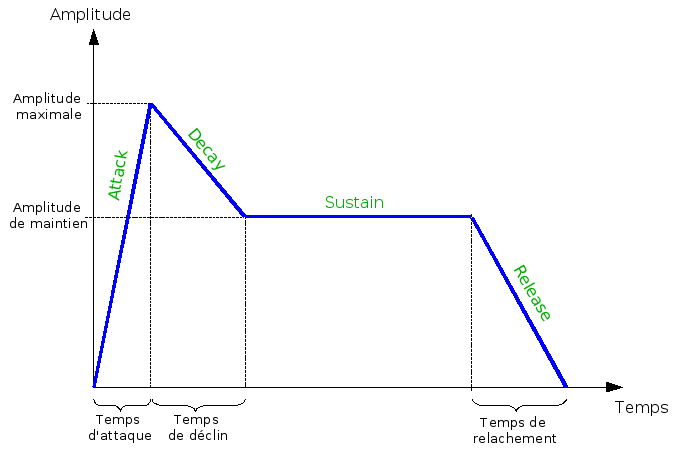
\includegraphics[height=6cm]{images/ADSR.png}
        \caption{Enveloppe sonore ADSR: modèle théorique}
    \end{minipage}\hfill
    \begin{minipage}[b]{0.48\linewidth}
        \centering 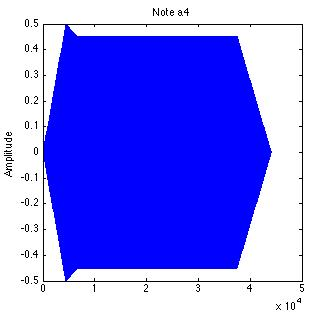
\includegraphics[height=6cm]{images/OurADSR.jpg}
        \caption{Affichage d'un de nos fichiers wave contenant une note lissée}
    \end{minipage}
\end{figure}

\section{Limitation du programme et difficultés perçues}
\subsection{Limitation du programme}
Une amélioration de notre programme serait la gestion des erreurs, 
puisque il arrive très souvent qu'une partition ou une musique soit mal écrite dans le fichier .dj.oz.
Il serait donc bien de retourner un message d'erreur expliquant que la partition est mal formatée 
plutôt que de laisser le programme se planter.
La seule erreur qui a été gérée est le cas où l'instrument n'existe pas (ou le cas où l'instrument
existe mais pas la note correspondante. Par exemple, il n'existe pas de note $g2$ pour 
l'instrument \textit{bassdist}). Dans ce cas nous retournons un message
d'erreur et remplaçons la son de l'instrument par une note pure.

\subsection{Difficultés rencontrées}
\subsubsection{Durée de compilation}
Il est difficile de réaliser un code efficace en terme de rapidité. Nous avons en effet une
vingtaine de fonctions s'appelant souvent entre elles et manipulant des listes
ou des records de taille assez conséquente. Nous avons essayé d'optimiser au mieux notre
code en utilisant le plus possible des fonctions résursives terminales.

\subsubsection{Compréhension des consignes}
Comme annoncé, une des parties les plus difficiles du projet consiste à 
comprendre les consignes. On se perd facilement parmis toutes les définitions
(partition, voix, échantillon, musique, morceau, vecteur audio, etc) et on finit
par ne plus savoir si tel ou tel fonction a besoin d'une partition ou d'une musique
en argument. Pour pallier au mieux à ce problème, nous avons essayé de commenter
chaque fonction en décrivant brièvement l'input et l'output. 
\newpage

\end{document}